\documentclass{../bredelebeamer}
\usepackage{multirow}
\usepackage{pdfpages}
\usepackage{braket,bigstrut}
\usepackage{palatino}
\usepackage{multicol,bigstrut}
\usepackage{listings}
\usepackage{tikz}
\usepackage{booktabs}
\usepackage{amsmath,amssymb,amsfonts,cancel,physics,siunitx}
\usetikzlibrary{positioning,shadows,backgrounds,calc}%
\setbeamercolor{footnote mark}{fg=black}
\setbeamercolor{footnote}{fg=black}


\renewcommand{\baselinestretch}{0.9}

\usepackage[backend=bibtex8,style=authortitle,autocite=footnote]{biblatex}
%\addbibresource{../../references.bib}

\renewbibmacro*{cite:title}{%
	\printtext[bibhyperref]{%
		\printfield[citetitle]{labeltitle}%
		\setunit{\space}%
		\printtext[parens]{\printdate}%
	}%
}

\renewcommand{\figurename}{{\bf Fig.}}
\usefonttheme{serif} % default family is serif

\renewcommand{\baselinestretch}{0.9}

\title[]{Interference effects}
\subtitle{}
\author[Cristian F. Rodríguez]{
	$ $\\
	Cristian Fernando Rodríguez Cruz\\
	$ $\\
	$ $\\
	Authors:\\
	A. Flórez\inst{1}, \textcolor{Framableu}{\textbf{C. Rodriguez}}\inst{1}, J. Reyes-Vega\inst{1},\\
	J. Jones-Pérez\inst{2}. \\
    $ $\\
	$ $\\
}

\institute[Uniandes]{\inst{1} Universidad de los Andes\and
\inst{2} Pontificia Universidad Católica del Perú 
}
\date{\today}
\lstset{language=C++,
  basicstyle=\ttfamily,
  keywordstyle=\color{blue}\ttfamily,
  stringstyle=\color{red}\ttfamily,
  commentstyle=\color{green}\ttfamily,
  morecomment=[l][\color{magenta}]{\#}
}

\begin{document}
\frame{\titlepage}

\begin{frame}{Two body scattering}{CM-Frame}
    Consider the process 
    \begin{equation}
        A(\va*{p}_1) + B(\va*{p}_2) \longrightarrow C(\va*{p}_3) + D(\va*{p}_4),
    \end{equation}
    \begin{center}
        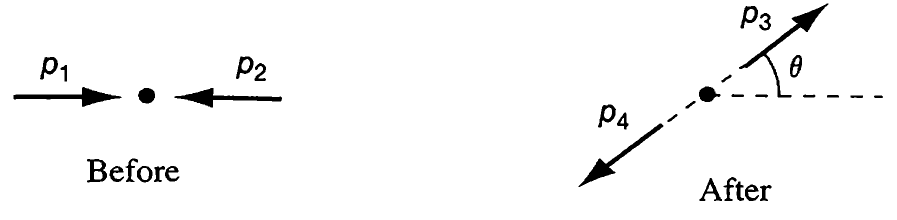
\includegraphics[width=0.6\textwidth]{scatter.png}
    \end{center}

    From the Golden Rule, the cross section is given by
    \begin{equation}
        \sigma = \frac{S (2\pi)^4}{4\sqrt{(\va*{p}_1\cdot\va*{p}_2)^2 - (m_1m_2)^2}}\int \abs{\mathcal{M}}^2\delta^{(4)}(p_1 + p_2 - p_3 - p_4)\frac{d^3\va*{p}_3}{(2\pi)^3 2E_3}\frac{d^3\va*{p}_4}{(2\pi)^3 2E_4}.
    \end{equation}
    But, in the CM frame, $\va*{p}_1 + \va*{p}_2 = 0$, where
    \begin{gather}
        \sqrt{(\va*{p}_1\cdot\va*{p}_2)^2 - (m_1m_2)^2} = E_1E_2 \abs{\va*{p}_1},
        \\
        \delta^{(4)}(p_1 + p_2 - p_3 - p_4) = \delta\left(
            E_1 + E_2 - E_3 - E_4
        \right)
        \delta^{(3)}(\va*{p}_3 + \va*{p}_4).
    \end{gather}
    Thus 
    \begin{equation}
        \sigma = \left(\frac{1}{8\pi}\right)^2 \frac{S}{(E_1E_2) \abs{\va*{p}_1}}\int \abs{\mathcal{M}}^2
        \frac{\delta\left(
            E_1 + E_2 - \sqrt{\va p_3^2 + m_3^2} - \sqrt{\va p_3^2 + m_4^2}
        \right)}{\sqrt{\va p_3^2 + m_3^2}\sqrt{\va p_3^2 + m_4^2}} \dd \va p_3
    \end{equation}
\end{frame}

\begin{frame}{Two body scattering}{CM-Frame}
    Integrating over the radial part $\abs{\va p_3}$, we get
    \begin{equation}
        \sigma = \left(\frac{1}{8\pi}\right)^2 \frac{S |\va*{p}_3|}{(E_1 +E_2)^2 \abs{\va*{p}_1}} \int \abs{\mathcal{M}}^2 \dd\Omega,
    \end{equation}
    with 
    \begin{equation}
        |\va*{p}_3| = \frac{1}{2} \frac{\sqrt{((E_1+E_2)^2 - m_3^2 -m_4^2)^2- 4m^2_3m^2_4} }{E_1+E_2},
    \end{equation}
    the outgoing momentum in the CM frame.

    $$ $$

    We prefer work with differential cross section as
    \begin{equation}
        \frac{\dd \sigma}{\dd \Omega} = \frac{1}{64\pi^2} \frac{S }{(E_1 +E_2)^2 } \frac{|\va*{p}_3|}{\abs{\va*{p}_1}} \abs{\mathcal{M}}^2.
    \end{equation}
   

    Note that at this point, we don't need to know the explicit form of the matrix element $\mathcal{M}$, so it is a generic result.
\end{frame}

\begin{frame}{Two body scattering}{CM-Frame}
    Defining $\sqrt s = E_1 + E_2$, we have
    \begin{equation}
        |\va*{p}_3| = \frac{1}{2} \frac{\sqrt{(s - m_3^2 -m_4^2)^2- 4m^2_3m^2_4} }{s}, \quad  |\va*{p}_1|\frac{1}{2} \frac{\sqrt{(s - m_1^2 -m_2^2)^2- 4m^2_1m^2_2} }{s}.
    \end{equation}
    so the differential cross section is
    \begin{equation}
        \frac{\dd \sigma}{\dd \Omega} = \frac{1}{64\pi^2} \frac{S }{s } 
        \sqrt{\frac{(s - (m_3 + m_4)^2)(s - (m_3 - m_4)^2)}{(s - (m_1 + m_2)^2)(s - (m_1 - m_2)^2)}}
        \abs{\mathcal{M}}^2.
    \end{equation}
    
    In general, there are three Lorentz-invariant useful kinematical variables to describe the scattering process, known as Mandelstam variables:
    \begin{align}
        \hat s &= (p_1 + p_2)^2 = (p_3 + p_4)^2,\\
        \hat t &= (p_1 - p_3)^2 = (p_2 - p_4)^2,\\
        \hat u &= (p_1 - p_4)^2 = (p_2 - p_3)^2.
    \end{align}
    In the CM-frame, $\hat s = s = (E_1+E_2)^2$.
\end{frame}

\begin{frame}
    
\end{frame}
\end{document}